\section{Aims and Objectives}
% Load graphicx package in preamble if not already loaded
\graphicspath{{./images/}}

\subsection{Primary Aim}
This research aims to deepen our understanding of spatially and demographically stratified heat-health interactions in Johannesburg, developing evidence-based approaches to mitigate health risks from rising urban temperatures. By examining the complex interplay between urban heat, socioeconomic factors, and health outcomes, this project seeks to bridge critical knowledge gaps in urban climate-health research within the African context, with potential applications for similar urban environments globally.

\subsection{Specific Objectives}
This research is structured around three interconnected objectives that progress from descriptive analysis to explanatory insights and ultimately to predictive capabilities:

\subsubsection{Objective 1: Intra-urban Heat Vulnerability Mapping}
The first objective centres on comprehensive spatial vulnerability assessment to identify patterns of heat risk across Johannesburg's diverse urban landscape. This mapping process will examine how historical urban development patterns, particularly those influenced by apartheid-era planning, continue to shape contemporary heat vulnerability. Through this assessment, we will identify priority intervention areas and quantify multidimensional vulnerability patterns with particular emphasis on socio-spatial inequities. This objective will result in detailed vulnerability characterization that can directly inform targeted urban planning and public health interventions.

\subsubsection{Objective 2: Heat-Health Dynamics Exploration}
Building on the vulnerability assessment, the second objective aims to unravel complex heat-health relationships by investigating the underlying physiological mechanisms through which heat exposure affects human health. Through a two-stage modelling approach, we will first generate hypotheses about key physiological pathways and then systematically test these hypotheses using targeted feature engineering. This component will focus particularly on metabolic, renal, and inflammatory responses to heat stress, examining how these systems interact across multiple temporal scales. 

The research will explore non-linear climate-health interactions across different temperature thresholds while distinguishing between immediate (0-24 hours), short-term (1-7 days), and medium-term (7-30 days) physiological effects. By applying interpretable machine learning techniques with clinically validated pathway diagrams, we seek to establish causal mechanisms that explain differential vulnerability between population groups and identify critical intervention points for health protection during heat events. This explanatory approach moves beyond simple statistical associations to provide mechanistic insights to inform targeted clinical and public health responses.

\subsubsection{Objective 3: Stratified Heat-Health Prediction Modeling}
The final objective leverages insights from the previous components to develop predictive frameworks for heat-related health outcomes in Johannesburg. These predictive capabilities will be stratified both geographically and demographically to account for differential vulnerability across the city's diverse population. The objective seeks to identify specific risk conditions at various temperature thresholds, enabling the development of targeted early warning systems. Special attention will be given to demographic-specific risk stratification for vulnerable populations, including the elderly, those with pre-existing conditions, and communities with limited adaptive capacity. The resulting predictive tools will provide actionable intelligence for healthcare systems and emergency response planning.

\begin{figure}[h]
    \centering
    % Adding a white background rectangle to prevent text showing through
    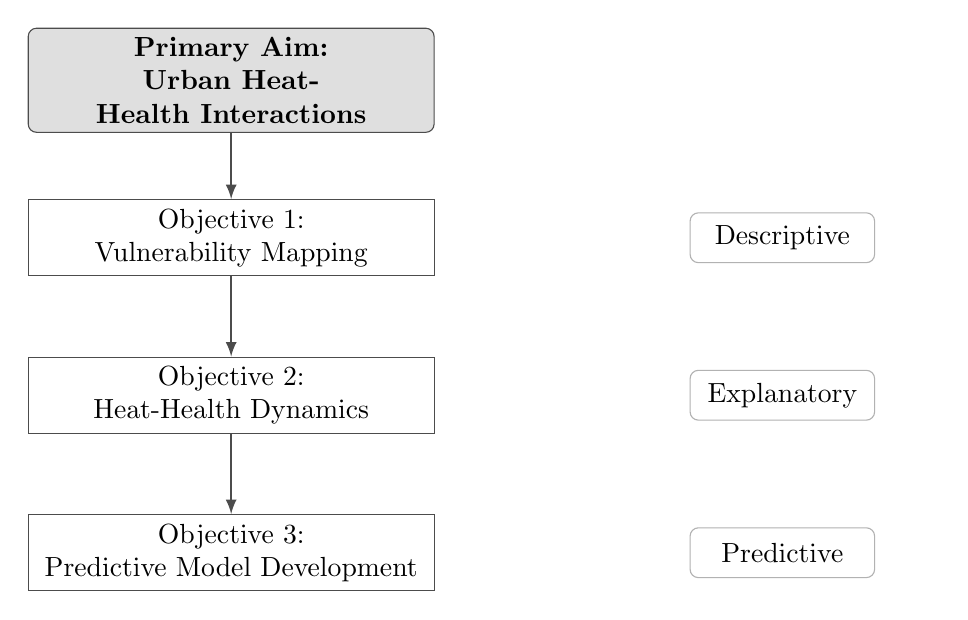
\begin{tikzpicture}[
        block/.style={rectangle, draw, rounded corners=3pt, text width=14em, text centered, minimum height=2.5em, font=\bfseries, fill=gray!15, draw=black!70},
        objective/.style={rectangle, draw, text width=14em, text centered, minimum height=2.5em, draw=black!70},
        arrow/.style={thick,->,>=stealth, draw=black!70},
        label/.style={rectangle, draw, rounded corners=3pt, fill=white, text width=6em, text centered, minimum height=1.8em, draw=black!30}
    ]
    
    % Add background rectangle to prevent text showing through
    \fill[white] (-1,-6.5) rectangle (9,0.5);
    
    % Primary Aim block with darker fill
    \node[block, fill=gray!25] (aim) at (0,0) {Primary Aim:\\Urban Heat-Health Interactions};
    
    % Objectives with distinctive styling
    \node[objective, fill=white] (obj1) at (0,-2) {Objective 1:\\Vulnerability Mapping};
    \node[objective, fill=white] (obj2) at (0,-4) {Objective 2:\\Heat-Health Dynamics};
    \node[objective, fill=white] (obj3) at (0,-6) {Objective 3:\\Predictive Model Development};
    
    % Arrows with slight curve for visual interest
    \draw[arrow, -latex] (aim) -- (obj1);
    \draw[arrow, -latex] (obj1) -- (obj2);
    \draw[arrow, -latex] (obj2) -- (obj3);
    
    % Labels with better positioning and styling
    \node[label] at (7,-2) {Descriptive};
    \node[label] at (7,-4) {Explanatory};
    \node[label] at (7,-6) {Predictive};
    
    \end{tikzpicture}
    \caption{Hierarchical framework of research objectives showing progression from descriptive to predictive approaches.}
    \label{fig:aims_objectives}
\end{figure}

Together, these three objectives form an integrated research framework that addresses the spatial dimension (identifying vulnerable areas), the physiological dimension (understanding underlying mechanisms), and the temporal dimension (developing predictive capabilities). This multi-dimensional approach will provide a comprehensive understanding of heat-health interactions in Johannesburg, with implications for urban planning, public health interventions, and climate adaptation strategies. The research design intentionally builds each objective upon the findings of the previous one, creating a cohesive analytical pathway from vulnerability characterization to mechanistic understanding to practical solution development. This progression from descriptive to explanatory to predictive aims reflects the holistic nature of the heat-health challenge and enables development of targeted, evidence-based interventions.